\documentclass[11pt]{article}

% Style follows the user's EDU498 Minecraft Identity mini-unit pattern:
% compact article layout, color-forward headings, simple TikZ figures, and table-rich reflection.
\usepackage[margin=0.6in]{geometry}
\usepackage[T1]{fontenc}
\usepackage[utf8]{inputenc}
\usepackage{lmodern}
\usepackage{array}
\usepackage{booktabs}
\usepackage{enumitem}
\usepackage{hyperref}
\usepackage{longtable}
\usepackage{parskip}
\usepackage{ragged2e}
\usepackage{setspace}
\usepackage{tabularx}
\usepackage{titlesec}
\usepackage[table]{xcolor}
\usepackage{tikz}
\usepackage[most]{tcolorbox}
\usetikzlibrary{arrows.meta,positioning,shapes.geometric,calc}

\definecolor{PrimaryRed}{HTML}{8B1E1E}
\definecolor{SoftBlue}{HTML}{DDEEFF}
\definecolor{DarkGray}{HTML}{333333}
\definecolor{SoftGreen}{HTML}{EEF6F2}
\definecolor{SoftGold}{HTML}{FFF6E6}
\definecolor{SoftPurple}{HTML}{F7F2FA}
\definecolor{SoftRose}{HTML}{FCEEEF}
\definecolor{PresentGreen}{HTML}{2E7D32}
\definecolor{PartialOrange}{HTML}{B26A00}
\definecolor{MissingRed}{HTML}{B3261E}

\hypersetup{colorlinks=true,linkcolor=black,urlcolor=black,citecolor=black}
\setlength{\parindent}{0pt}
\setstretch{1.12}
\newcolumntype{Y}{>{\RaggedRight\arraybackslash}X}
\newcolumntype{L}[1]{>{\RaggedRight\arraybackslash}p{#1}}
\setlist[itemize]{topsep=2pt,itemsep=1pt,parsep=0pt,partopsep=0pt,leftmargin=1.2em}
\setlist[enumerate]{topsep=2pt,itemsep=2pt,parsep=0pt,partopsep=0pt,leftmargin=1.3em}
\titleformat{\section}{\large\bfseries\color{PrimaryRed}}{}{0em}{}
\titleformat{\subsection}{\normalsize\bfseries}{\thesubsection}{0.5em}{}

\newcommand{\Present}{\textbf{\textcolor{PresentGreen}{Present}}}
\newcommand{\Partial}{\textbf{\textcolor{PartialOrange}{Partial}}}
\newcommand{\Missing}{\textbf{\textcolor{MissingRed}{Missing}}}

\newtcolorbox{ReflectionBox}{
  colback=SoftPurple,
  colframe=PrimaryRed,
  boxrule=0.8pt,
  arc=2mm,
  left=1.5mm,
  right=1.5mm,
  top=1.2mm,
  bottom=1.2mm
}

\newtcolorbox{TakeawayBox}{
  colback=SoftGreen,
  colframe=DarkGray,
  boxrule=0.6pt,
  arc=2mm,
  left=1.5mm,
  right=1.5mm,
  top=1mm,
  bottom=1mm
}

\begin{document}

{\LARGE\bfseries\color{PrimaryRed} Indicator 13 Checklist Review and Reflection\par}
{\large ED452C --- Sample High-School IEP Transition Analysis\par}
\vspace{0.2em}
{\normalsize Student: James (Jimmy), age 17, Grade 10 \hfill Reviewer: Piter\par}

\vspace{0.55em}
\begin{center}
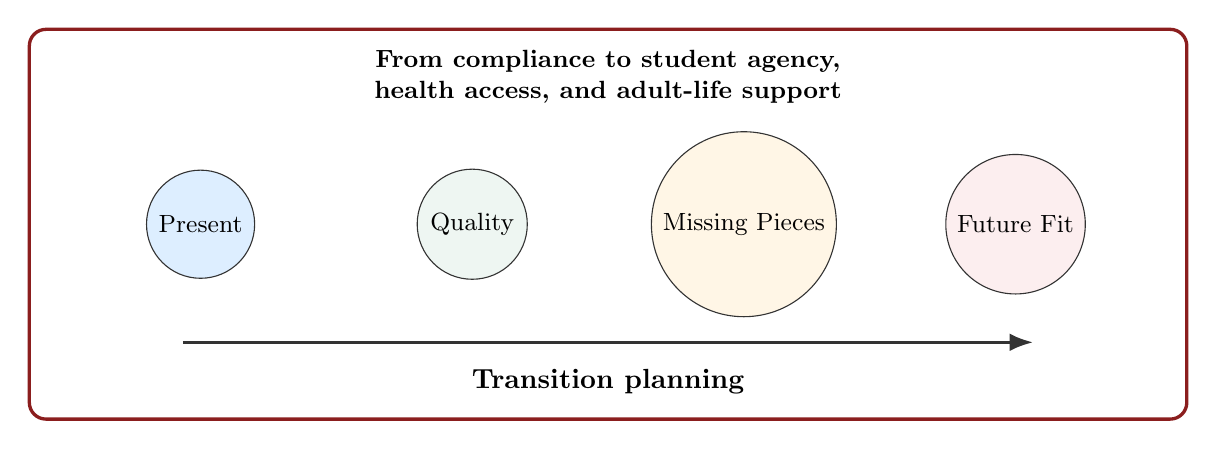
\begin{tikzpicture}[scale=1.5, every node/.style={font=\small, align=center}]
  % Outer frame
  \draw[rounded corners=6pt, very thick, PrimaryRed] (-4.9,-1.55) rectangle (4.9,1.75);

  % Top message
  \node[font=\small\bfseries, align=center, text width=9.9cm] at (0,1.35)
  {From compliance to student agency, health access, and adult-life support};

  % Four review lenses
  \node[circle, fill=SoftBlue,  draw=DarkGray, minimum size=1.28cm] at (-3.45,0.1) {Present};
  \node[circle, fill=SoftGreen, draw=DarkGray, minimum size=1.28cm] at (-1.15,0.1) {Quality};
  \node[circle, fill=SoftGold,  draw=DarkGray, minimum size=1.35cm] at 
  (1.15,0.1) {Missing Pieces};
  \node[circle, fill=SoftRose,  draw=DarkGray, minimum size=1.35cm] at 
  (3.45,0.1) {Future Fit};

  % Bottom process line, separated from circles
  \draw[very thick, -{Latex[length=3mm]}, DarkGray] (-3.6,-0.9) -- (3.6,-0.9);

  % Process label below the arrow, not on top of it
  \node[font=\bfseries, fill=white, inner sep=2pt] at (0,-1.23)
  {Transition planning};
\end{tikzpicture}
\end{center}

\begin{ReflectionBox}
\textbf{Guiding claim.} A transition section should not only prove that required items are present. It should show how the student is being prepared to move into adult life with voice, support, self-advocacy, dignity, and realistic access to future education, work, community, health, and relationships.
\end{ReflectionBox}

\section{Purpose and Course Lens}

This review applies the Indicator 13 transition checklist to the course-provided high-school sample IEP for Jimmy, a 17-year-old student in Grade 10. The assignment asks for a completed checklist and a reflection that discusses what was present, the quality of the information present, and what additional information would strengthen alignment between the transition section and the rest of the IEP. It also asks whether the transition section is designed appropriately to meet the student's goals and objectives.

My course lens centers on neurodivergent learners, chronically ill students, students experiencing depression or anxiety, trauma-experienced students, culturally and linguistically diverse students, and students with intersecting identities. I do not read the sample as evidence that Jimmy has depression or a trauma history; the IEP does not document that. However, the review uses depression-responsive and trauma-informed thinking because transition planning for students with special needs should anticipate stress, fatigue, social vulnerability, medical complexity, and the emotional weight of adult-life transitions before a crisis occurs.

Jimmy's IEP contains rich present-level information. He is identified as having Other Health Impairment and Speech Language Impairment; he has Prader-Willi syndrome, significant health and food-safety needs, language delays, academic support needs, social goals, counseling services, and a career interest connected to early childhood education (Sample IEP, pp. 2--12). The strongest parts of the IEP protect access and safety. The weaker parts are where protection needs to become a future-ready agency.

\newpage
\section{Completed Indicator 13 Checklist}

\begin{center}
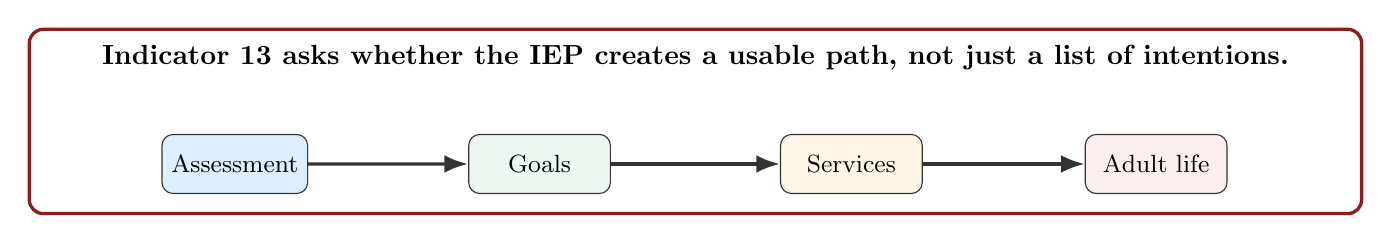
\begin{tikzpicture}[scale=1.8, every node/.style={font=\small, align=center}]
  \draw[rounded corners=5pt, very thick, PrimaryRed] (-4.7,-0.1) rectangle (4.7,1.2);
  \node[draw=DarkGray, fill=SoftBlue, rounded corners=4pt, minimum width=1.8cm, minimum height=0.75cm] (a) at (-3.25,0.25) {Assessment};
  \node[draw=DarkGray, fill=SoftGreen, rounded corners=4pt, minimum width=1.8cm, minimum height=0.75cm] (b) at (-1.1,0.25) {Goals};
  \node[draw=DarkGray, fill=SoftGold, rounded corners=4pt, minimum width=1.8cm, minimum height=0.75cm] (c) at (1.1,0.25) {Services};
  \node[draw=DarkGray, fill=SoftRose, rounded corners=4pt, minimum width=1.8cm, minimum height=0.75cm] (d) at (3.25,0.25) {Adult life};
  \draw[very thick, -{Latex[length=3mm]}, DarkGray] (a) -- (b);
  \draw[very thick, -{Latex[length=3mm]}, DarkGray] (b) -- (c);
  \draw[very thick, -{Latex[length=3mm]}, DarkGray] (c) -- (d);
  \node[align=center, font=\bfseries] at (0,1.0) {Indicator 13 asks whether the IEP creates a usable path, not just a list of intentions.};
\end{tikzpicture}
\end{center}

\footnotesize
\rowcolors{2}{white}{SoftBlue!35}
\begin{longtable}{L{0.16\textwidth} L{0.055\textwidth} L{0.07\textwidth} L{0.63\textwidth}}
\toprule
\textbf{Checklist Item} & \textbf{Status} & \textbf{Evidence} & \textbf{IEP Quality Review} \\
\midrule
\endfirsthead
\toprule
\textbf{Checklist Item} & \textbf{Status} & \textbf{Evidence} & \textbf{IEP Quality Review} \\
\midrule
\endhead
Education/training postsecondary goal & \Present & p. 8 & The goal states that Jimmy will attend college to take courses focused on Early Childhood Education. This is future-oriented and connected to a named field. It should be strengthened by naming disability services access, accommodation use, campus supports, and the type of postsecondary setting that is realistic. \\

Employment postsecondary goal & \Present & p. 8 & The employment goal states that Jimmy wants competitive employment in a daycare facility. This is clear and meaningful. It needs stronger work-based experiences, job-shadowing, supervised volunteer practice, employer communication routines, and health/safety planning for childcare settings. \\

Independent living goal, when appropriate & \Partial & p. 8 & Jimmy states that he wants to live in Chicago with friends, while his mother notes that he'll need lifelong support. The student voice is valuable, but the goal isn't operationalized. It needs specific supports for food safety, health routines, transportation, budgeting, community safety, and supported decision-making. \\

Age-appropriate transition assessment & \Partial & pp. 5, 8 & The IEP includes interests, parent concerns, strengths, and student preferences. Still, it doesn't name a formal transition assessment, vocational interest inventory, adaptive living assessment, student interview tool, or self-determination measure (the largest quality gaps). \\

Transition needs based on strengths, preferences, and interests & \Present & p. 8 & The IEP identifies needs in math computation, reading comprehension, self-advocacy, and researching credentials for early childcare work. This connects to Jimmy's adult goals, but self-advocacy has no matching annual goal or explicit instructional plan. \\

Course of study aligned with postsecondary goals & \Partial & p. 8 & The IEP lists a Regents Diploma pathway with special education support. This isn't career-specific enough. The plan should include child development, career and technical education exposure, job-shadowing, or community-based early childhood experiences. \\

Annual goals aligned to transition needs & \Partial & pp. 8--9 & Reading, writing, math, and language goals support college and workplace readiness. However, the plan is missing needs, such as an annual goal for self-advocacy, health self-management, accommodation use, regulation, or independent living, which are essential for the transition. \\

Transition services/activities across required areas & \Partial & p. 12 & The plan includes instruction in memorization strategies, language services, appointment-making, career research, budgeting, and no current functional vocational assessment. The activities need clearer timelines, responsible adult roles, measurable outcomes, community settings, and student-led practice. \\

Student invited to transition IEP meeting & \Missing & p. 2 & The meeting attendance doesn't list Jimmy. Because the IEP includes transition planning, the documentation should show that Jimmy was invited or that other steps were taken to gather and consider his preferences and interests. \\

Outside agency invited with consent when appropriate & \Missing & pp. 2, 12 & No adult-service agency, vocational rehabilitation representative, postsecondary disability services contact, or community agency is documented. Given Jimmy's age, health needs, employment goal, and likely lifelong support needs, agency coordination should be considered. \\

\bottomrule
\end{longtable}
\normalsize

\begin{TakeawayBox}
\textbf{Checklist snapshot.} The IEP includes many transition elements. However, the pattern is mostly \textit{partial}: the plan names adult goals, but it does not yet fully show the assessment base, student participation, agency coordination, or adult-life skill instruction needed to make those goals usable.
\end{TakeawayBox}

\section{What Was Present}

Several important Indicator-13 elements were present. Jimmy's IEP includes postsecondary goals in education/training, employment, and independent living. His education/training goal is to attend college or university for early childhood education courses, and his employment goal is competitive employment in a daycare facility. His independent living statement includes his own goal of living in Chicago with friends, while also documenting his mother's concern that he will need some level of lifetime support (Sample IEP, p. 8). \textit{This is important because it shows both student voice and family knowledge}.

The IEP also includes a transition needs section. Jimmy needs to increase math computation and reading comprehension for college success, increase self-advocacy skills, and research the credentials necessary to become an early childcare worker (Sample IEP, p. 8). His course of study includes general education courses needed for a Regents Diploma with special education supports in math, social studies, science, and English. \textit{Annual goals in reading, writing, mathematics, and speech/language connect at least indirectly to college and employment readiness (Sample IEP, pp. 8--9)}.

A major strength is that the IEP takes Jimmy's chronic health profile seriously. It includes extensive food-related precautions, temperature-regulation supports, supervision needs, counseling, speech/language therapy, a calculator, extended time, simplified directions, class notes, break periods, and staff training related to Prader-Willi syndrome (Sample IEP, pp. 3, 6--11). From an inclusion standpoint, \textit{these supports matter because they treat disability and chronic illness as part of learning access}.

The IEP also includes coordinated transition activities, such as instruction in memorization strategies, speech/language services, appointment-making, internet, and career materials research regarding Early Childhood Education careers, budgeting, and a statement that a functional vocational evaluation isn't needed at this time (Sample IEP, p. 12). \textit{These activities show that the team is trying to connect school skills to post-school life}.

\section{Quality of the Information Present}

The quality of the transition section is mixed. The IEP has a credible foundation, but it is stronger as a school-management plan than as an adult-transition plan. It protects Jimmy during the school day, but it does not yet clearly teach him how to understand, explain, request, and manage those supports in adult contexts.

The postsecondary goals are meaningful but not fully measurable in the strongest sense. ``Attend college or university'' and ``be competitively employed working in a daycare facility'' are understandable goals. However, they would be stronger if connected to specific transition assessments, disability-support planning, career exploration, and steps toward real-world participation. For example, the IEP could include a visit to a postsecondary disability services office, a supported interview with a childcare professional, or volunteer hours in a supervised early childhood setting.

The independent living goal needs the most development. Jimmy's desire to live in Chicago with friends matters because it shows imagination, preference, and agency. At the same time, the IEP itself recognizes that he will need support throughout his lifetime. A high-quality transition plan should not dismiss his goal but translate it into teachable steps: budgeting, safe transportation, food access routines, social decision-making, emergency communication, medication or health supports if applicable, and supported decision-making. Without these details, the independent living statement remains more aspirational than instructional.

\newpage
The IEP names self-advocacy as a transition need, but this is where quality drops. Self-advocacy does not appear as an annual goal. There is no clear plan for Jimmy to practice explaining his needs, asking for clarification, requesting accommodations, identifying when he is overwhelmed, or communicating health risks to new adults. This is especially important for neurodivergent and chronically ill students because adult systems usually require more self-initiation than K--12 school systems. A student who has been protected through adult management needs explicit instruction in how to participate in that protection.

The social-emotional information is also meaningful but underused. The IEP notes anxiety, mood regulation concerns, somatic complaints, social withdrawal, missed social cues, and the importance of peer relationships (Sample IEP, pp. 5--6). Yet, the transition plan does not strongly connect those needs to future college, workplace, or community situations. For students with depression, anxiety, trauma histories, or chronic illness, transitions can increase stress. A stronger plan would include a coping plan, a trusted adult network, scripts for help-seeking, predictable routines, and re-entry supports after absences or health-related disruptions.

\section{Additional Information That Would Strengthen the Transition Section}

The first major addition should be a named age-appropriate transition assessment. The IEP includes scattered transition-relevant information, but it does not identify the assessment tools or student interview process used to generate the goals. A stronger plan would include a dated transition interview, vocational interest inventory, adaptive living checklist, self-determination measure, and health self-management checklist. \textit{This would make the plan more defensible and more student-centered}.

The second addition should be a student-led transition component. Jimmy should be invited to the IEP meeting, and the IEP should document how his preferences were gathered if he did not attend. A short first-person statement could strengthen the transition section: ``My goal is to work with young children. I learn best when directions are broken down. I need help managing food and temperature safety. I want to learn how to ask for support without feeling embarrassed.'' \textit{This would make the plan feel less like adults planning around Jimmy and more like adults planning with him}.

The third addition should be explicit goals for self-advocacy, health self-management, and emotional regulation; these goals are transition skills. For example, Jimmy could work on identifying when he needs a break, using a script to request directions in another way, explaining his food and temperature needs to a trusted adult, or practicing how to contact a disability services office. These would align directly with his future college, employment, and living goals.

The fourth addition should be agency coordination. Given Jimmy's goal of college coursework, daycare employment, and supported adult living, the team should consider inviting vocational rehabilitation, postsecondary disability services, adult health/care coordination, or another relevant adult-service agency with appropriate consent. The IEP does not document this. \textit{Without agency coordination, families can be left to build the adult support bridge alone}.

The fifth addition should be trauma-informed and depression-responsive transition planning. This means designing predictable, dignity-preserving supports for students whose nervous systems, health histories, anxiety, or past school experiences may make transition stressful. The plan could include private correction, preparation before schedule changes, safe help-seeking routines, counseling continuity, and \textit{clear steps for what to do when the student feels overwhelmed}.

\section{Appropriateness of the Transition Section}

Overall, the transition section is \textit{partially appropriate} for Jimmy's goals and objectives. It is appropriate because it names postsecondary goals, connects those goals to academic and communication needs, identifies some coordinated activities, and includes extensive support for health and access. The team clearly understands that Jimmy's disability affects much more than academic performance; that is a strength.

However, the section is not fully appropriate if judged by whether it prepares Jimmy to carry support into adult life. The plan is heavily adult-managed. Adult supervision is necessary for safety, but transition planning should also show how Jimmy will gradually learn pieces of the routine himself. For example, if adults currently manage food access and temperature regulation, the transition plan should teach Jimmy how to identify safe foods, explain restrictions, notice overheating signs, carry emergency information, and ask for support in new settings.

The plan also needs a stronger employment bridge. Competitive employment in a daycare facility is a meaningful goal, but the IEP does not show enough direct exposure to childcare settings. For a student with language, health, social, and self-advocacy needs, the team should not wait until after high school to test whether this environment is accessible. Supported observation, job shadowing, volunteer experiences, and employer-simulation tasks would help the team determine what accommodations and skills Jimmy needs.

The independent living goal also needs a clearer balance between aspiration and support. Jimmy's goal to live with friends should not be dismissed as unrealistic, but it needs a structured pathway. This is where strengths-based transition planning matters. A strong team would ask: What part of this goal reflects belonging? What part reflects independence? What supports would allow Jimmy to experience friendship, community, and adult dignity safely? That question is more inclusive than simply deciding whether the goal is realistic.

\section{Concrete Recommendations}

\begin{enumerate}
  \item \textit{Add formal transition assessment evidence.} Include a dated transition interview, vocational interest inventory, adaptive living assessment, student preference profile, and health self-management checklist.
  \item \textit{Document student invitation and participation.} Invite Jimmy to the transition IEP meeting, document his attendance or input, and include a first-person transition statement.
  \item \textit{Add self-advocacy annual goals.} Write goals for requesting clarification, explaining accommodations, asking for breaks, and communicating health/safety needs.
  \item \textit{Strengthen the early childhood employment pathway.} Add job shadowing, supervised volunteer experiences, career interviews, and reflection prompts tied to daycare work expectations.
  \item \textit{Build health-management transition skills.} Teach Jimmy to identify food, temperature, fatigue, choking, and safety needs in ways that can transfer to college, work, transportation, and community settings.
  \item \textit{Include mental-health and trauma-informed supports.} Add predictable routines, coping strategies, trusted-adult contacts, counseling continuity, private support, and re-entry plans after illness or overwhelm.
  \item \textit{Coordinate with adult systems.} Consider vocational rehabilitation, postsecondary disability services, adult healthcare/care coordination, and supported living resources with appropriate consent.
\end{enumerate}

\newpage
\section{Conclusion}

This IEP has a meaningful transition foundation, but it needs stronger alignment between compliance and quality. The transition section includes postsecondary goals, a course of study, annual goals, services, and coordinated activities. It also reflects serious attention to chronic illness and school-day access. Those are important strengths. The central weakness is that the transition plan does not yet fully build Jimmy's adult-life agency. It protects him more than it teaches him how to participate in his own protection. For neurodivergent, chronically ill, depression-affected, trauma-experienced, and multiply identified students, transition planning must be more than a document that says where the student might go next. It must teach the student how to move into the future with support that is usable, respectful, and transferable.

\begin{ReflectionBox}
This transition section is partially appropriate but not complete. It should be revised so that Jimmy's goals for college, childcare employment, and adult living are supported by formal transition assessment, student-led planning, self-advocacy instruction, health self-management, emotional support, and adult-agency coordination.
\end{ReflectionBox}

\newpage
\section*{References}
\small
CASEL. (n.d.). \textit{What is the CASEL framework?} \url{https://casel.org/fundamentals-of-sel/what-is-the-casel-framework/}

ED452C. (n.d.). \textit{Indicator 13 Checklist Review Directions and Rubric}. Course handout.

Individuals with Disabilities Education Act, 34 C.F.R. \S\S 300.43, 300.320, 300.321. \url{https://sites.ed.gov/idea/regs/}

National Child Traumatic Stress Network. (n.d.). \textit{Trauma-informed care}. \url{https://www.nctsn.org/trauma-informed-care}

National Institute of Mental Health. (n.d.). \textit{Teen depression: More than just moodiness}. \url{https://www.nimh.nih.gov/health/publications/teen-depression}

Office of Special Education and Rehabilitative Services. (2017). \textit{A transition guide to postsecondary education and employment for students and youth with disabilities}. U.S. Department of Education. \url{https://sites.ed.gov/idea/files/postsecondary-transition-guide-may-2017.pdf}

Prader-Willi Syndrome Association USA. (n.d.). \textit{Sample Individualized Education Program (IEP)}. Sample high-school IEP.

\end{document}